% Carried over verbatim from monograph/main.tex (Study 1 record, 13 Sep 2026).
\chapter{Literal overlap and conservative duplicate grouping}\label{s1:ch:ch08_literal_overlap_and_conservative_duplica}

\section{Literal source-pixel overlap}

SIPaKMeD's recovered boxes permit a stronger question than shared parent identity. Let boxes $B_i$ and $B_j$ come from the same field. Their intersection is non-empty when
\begin{equation}
\max(x_i,x_j)<\min(x_i+w_i,x_j+w_j)
\quad\text{and}\quad
\max(y_i,y_j)<\min(y_i+h_i,y_j+h_j).
\end{equation}
The intersection-over-union is
\begin{equation}
\operatorname{IoU}(B_i,B_j)=\frac{|B_i\cap B_j|}{|B_i\cup B_j|}.
\end{equation}

Across 13,064 within-parent crop pairs, 2,185 share at least one pixel and the maximum IoU is 0.546. Under P1, 16.80$\pm$0.77\% of cross-split sibling pairs overlap and 52.62$\pm$1.97\% of test crops overlap at least one source pixel with a training crop. Both quantities are 0.00$\pm$0.00\% under P2 and P3.

\begin{figure}[H]
\centering
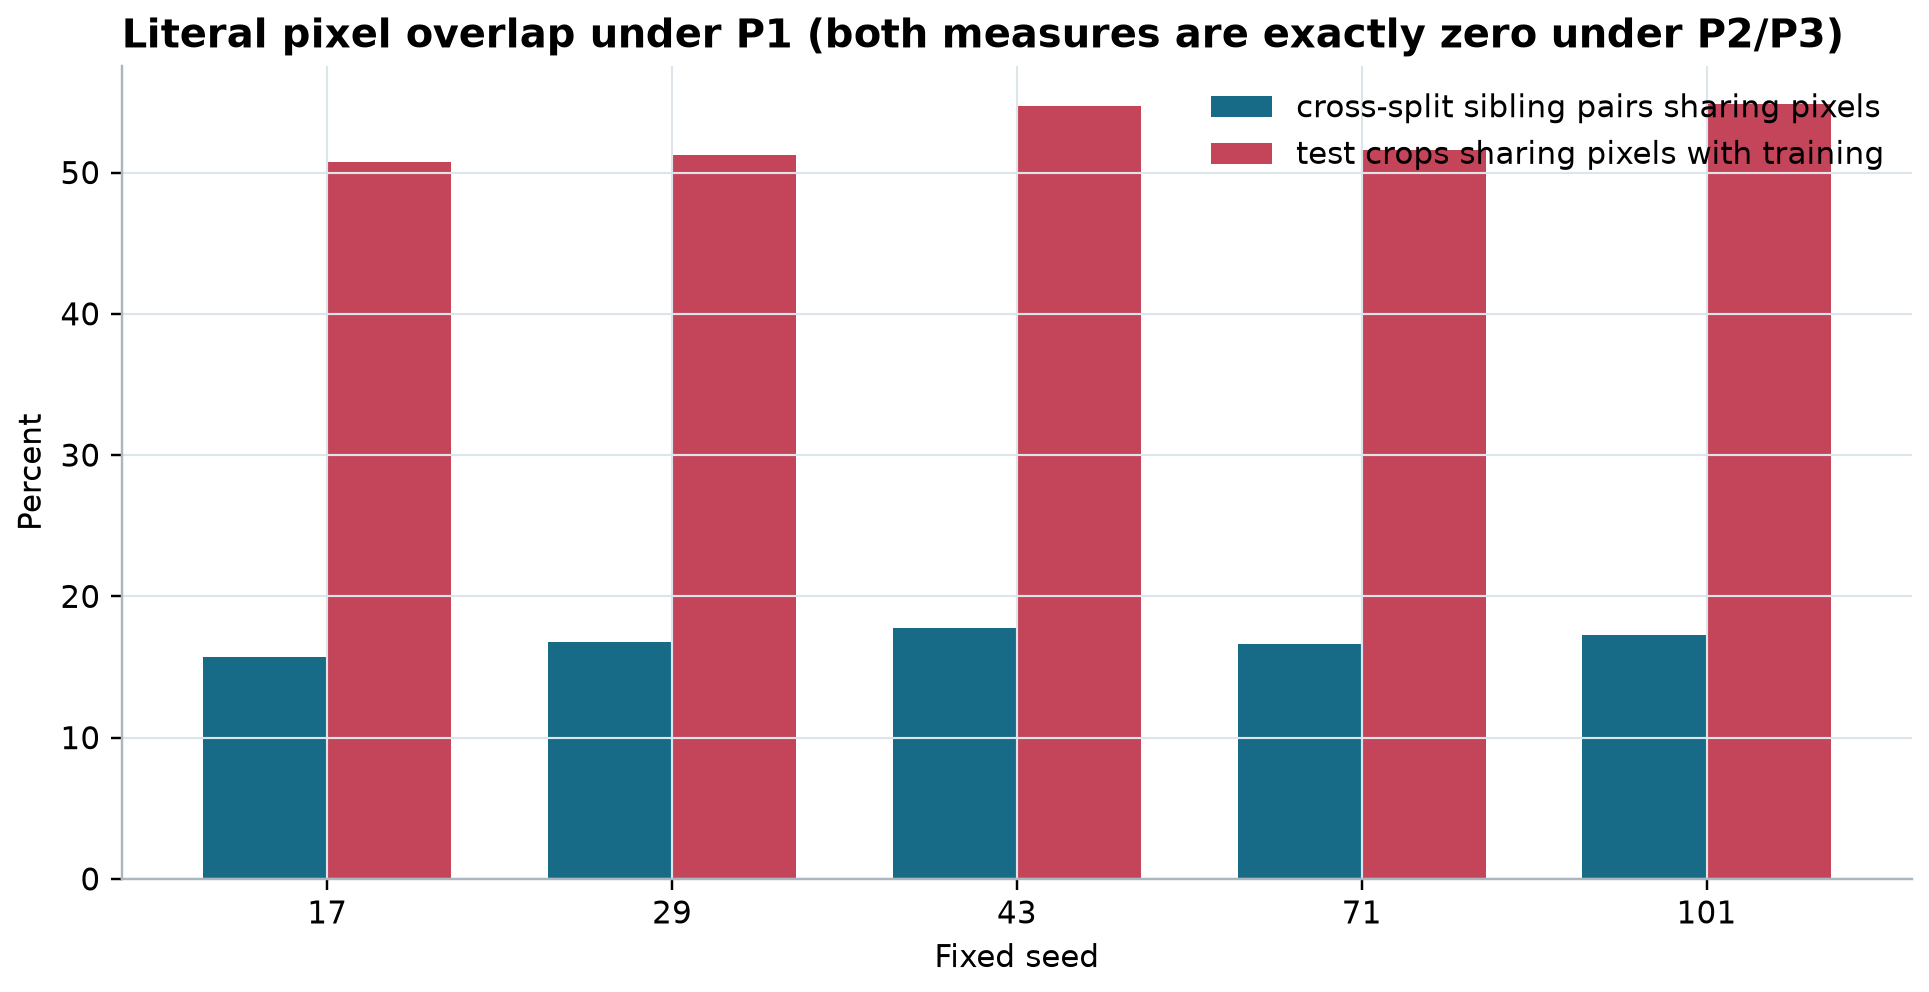
\includegraphics[width=0.9\textwidth]{literal_pixel_overlap.png}
\caption{Literal overlap for every P1 seed. The larger test-crop fraction answers a different question from the pair fraction: whether each test crop has at least one overlapping training sibling.}
\label{s1:fig:pixel-overlap}
\end{figure}

\section{Perceptual hashes and P3}

For each crop the implementation computes a 64-bit perceptual hash from the median-thresholded low-frequency $8\times8$ DCT block and a 64-bit difference hash from adjacent comparisons in an $8\times9$ downsample. Two crops become a candidate pair when they are pixel-exact or when both Hamming distances are at most six. Cross-parent candidate pairs are joined by union-find; each connected component becomes one P3 group.

At the frozen thresholds, the audit found 201 cross-parent candidate pairs. They connect 170 parent IDs into 74 components, the largest containing eight parents, and reduce 966 parents to 870 P3 groups. No pair is pixel-exact. A synthetic calibration detected all three injected transformations and rejected all 100 deterministic unrelated-parent negatives, yielding precision 1.00 and recall 1.00 on that calibration set.

\begin{figure}[H]
\centering
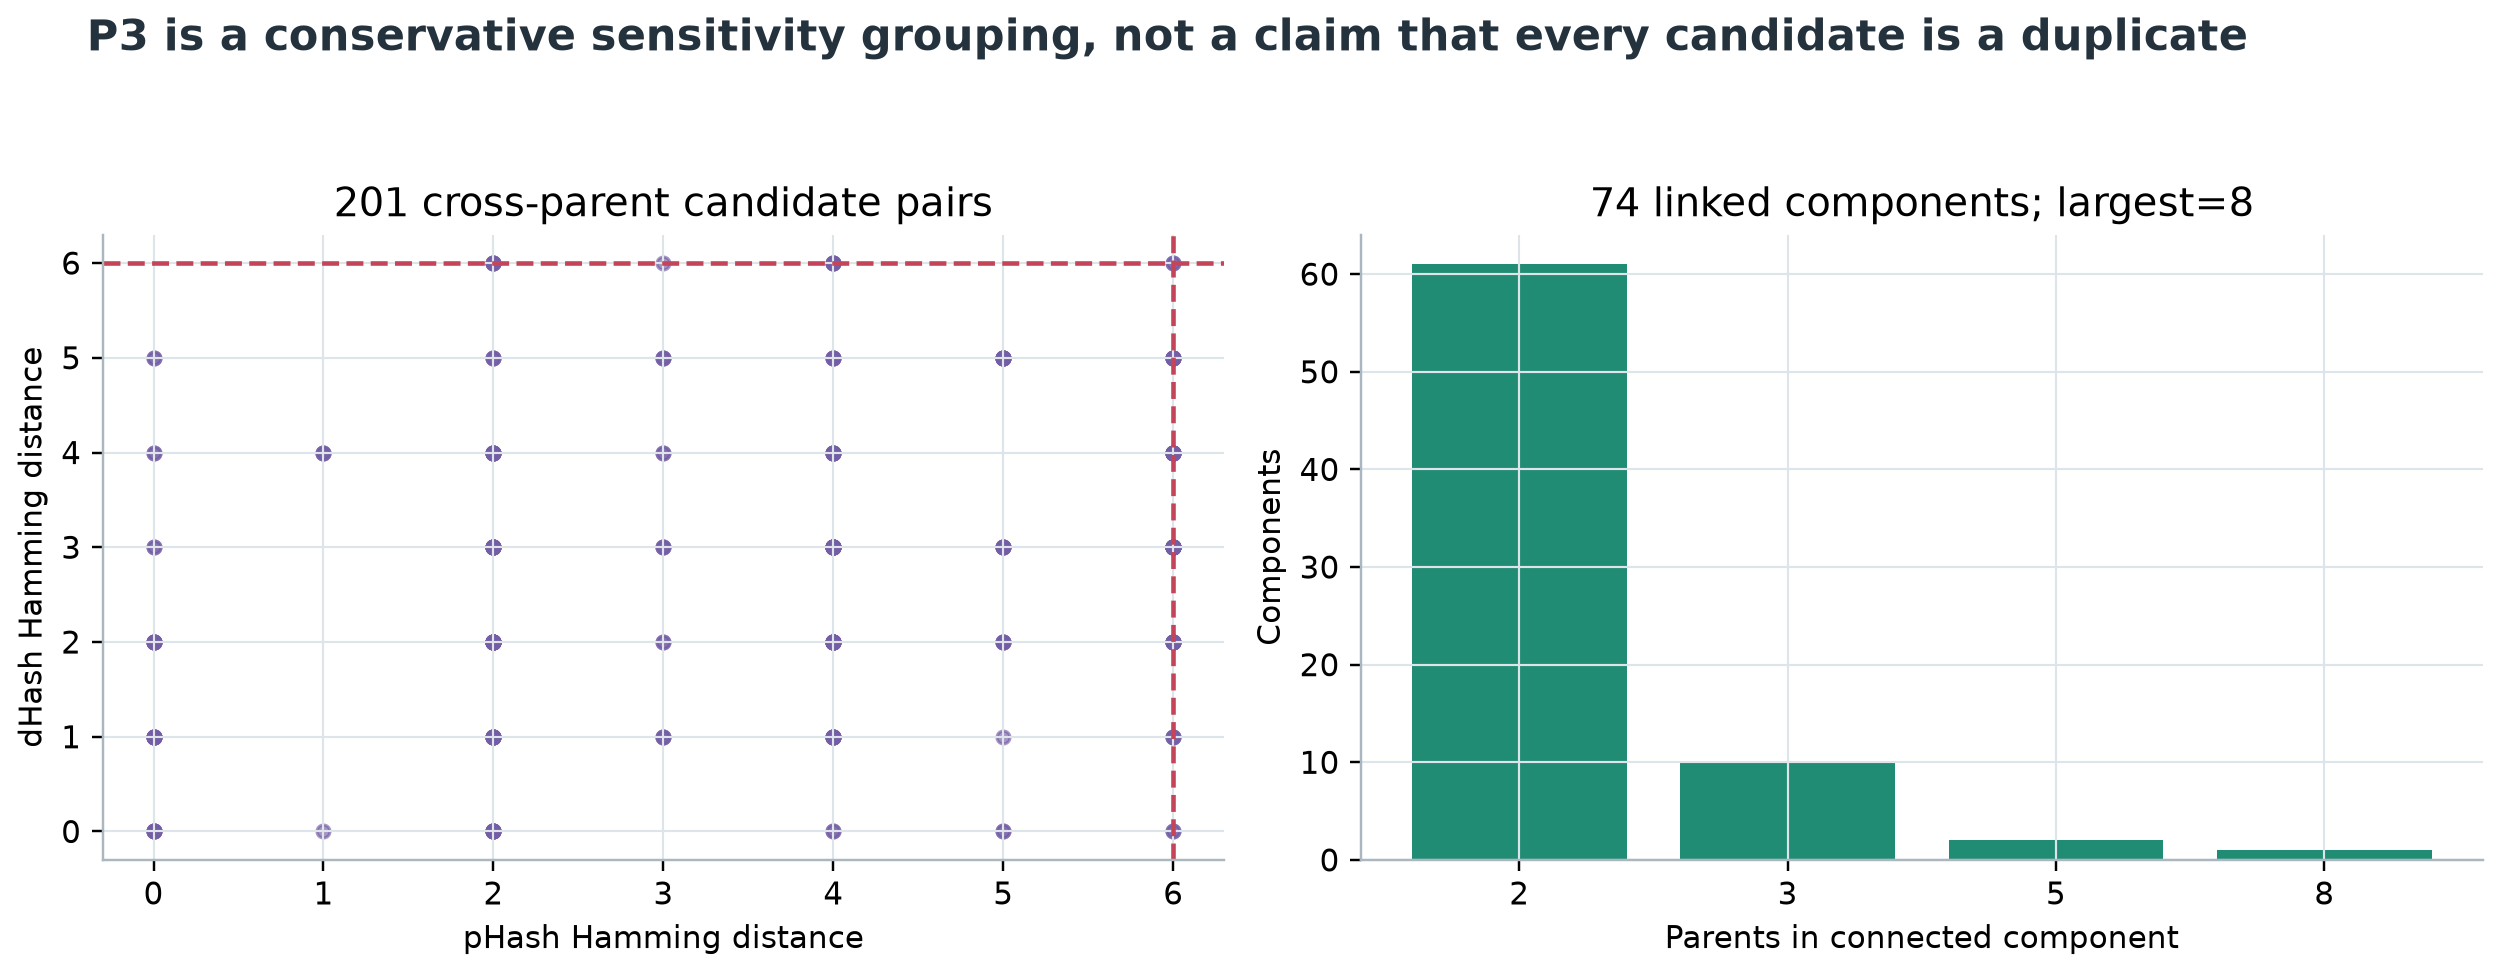
\includegraphics[width=\textwidth]{duplicate_audit.png}
\caption{Near-duplicate sensitivity audit. The thresholded candidates are used conservatively for grouping; they are not treated as ground-truth duplicate annotations.}
\label{s1:fig:duplicates}
\end{figure}

\begin{warningbox}{What the duplicate experiment did not do}
The broader planning idea mentioned a three-detector majority vote involving learned features. The frozen release implements only the pHash+dHash consensus audit and its synthetic calibration. Therefore the report does not claim a CNN/domain-encoder duplicate ensemble, human-confirmed duplicate truth, or general detector precision outside the calibration set.
\end{warningbox}
